% !TeX program = xelatex
% 编译方式：xelatex technical_report_v01.tex（建议连续编译两次以生成目录）
\documentclass[UTF8,a4paper,12pt]{ctexart}

\usepackage[left=2.7cm,right=2.7cm,top=2.5cm,bottom=2.5cm]{geometry}
\usepackage{graphicx}
\usepackage{booktabs}
\usepackage{array}
\usepackage{longtable}
\usepackage{enumitem}
\usepackage{float}
\usepackage{hyperref}
\hypersetup{colorlinks=true,linkcolor=black,urlcolor=blue,citecolor=black}
\setlist{nosep}
\setlength{\parindent}{2em}
\linespread{1.35}

% ===== 请在此处填写封面信息 =====
\newcommand{\reporttitle}{基于多传感器融合的无人机高精度目标定位系统}
\newcommand{\courseunit}{软件学院}
\newcommand{\majorname}{软件工程}
\newcommand{\membernames}{王博（组长）、李喆、胡艺琳、阳宇、吴嘉莹}
\newcommand{\advisorname}{\underline{\hspace{7.0cm}}}
\newcommand{\reportdate}{2026年8月24日\quad—\quad2026年9月18日}

\begin{document}

% ==================== 封面 ====================
\begin{titlepage}
  \centering
  \vspace*{0.8cm}
  
\includegraphics[width=0.68\textwidth]{assets/southeast_university_logo.png}\par
  \vspace{1.0cm}
  {\heiti\fontsize{32pt}{40pt}\selectfont 暑校实训项目文档\par}
  \vspace{1.4cm}
  {\zihao{-2}题\quad 目：\quad\bfseries \parbox[t]{0.76\textwidth}{\centering \reporttitle}\par}
  \vspace{1.2cm}
  {\zihao{3}\courseunit\quad 院（系）\qquad \majorname\quad 专业\par}
  \vspace{0.7cm}
  \begin{tabular}{@{}>{\raggedleft\arraybackslash}p{3.0cm}p{9.2cm}@{}}
    \zihao{3}组员姓名 & \zihao{3}\membernames\\[0.3cm]
    \zihao{3}指导教师 & \zihao{3}\advisorname\\[0.5cm]
  \end{tabular}\par
  \vspace{0.4cm}
  {\zihao{3}\reportdate\par}
\end{titlepage}

\pagenumbering{Roman}
\begin{center}
  {\heiti\zihao{2}诚信声明\par}
\end{center}
\vspace{1.2cm}
本报告由本项目组成员在指导教师指导下完成。我们承诺，报告中所述的项目过程、测试方法和结论均据实撰写；引用的资料、软件和技术文档均按规范标注。对于尚未完成实机闭环验证的内容，报告已明确其证据范围，不以规划指标、仿真结果或合成数据替代实测结论。
\vfill
\begin{flushright}
项目组：\membernames\\[0.5cm]
\reportdate
\end{flushright}
\clearpage

\tableofcontents
\clearpage

\begin{abstract}
\noindent\textbf{研究问题与项目目标：} 本报告面向无人机场景下的高精度外部静态目标定位需求，关注平台自身状态与外部目标位置如何在复杂环境中协同表达。我们的目标是构建一条从多源感知接入、坐标统一和融合估计，到可视化展示与实验归档的原型链路，并始终保持定位系统不直接干预飞行控制的安全边界。

\noindent\textbf{系统方案与核心工作：} 系统以机载视觉、UWB 测距、惯性信息和平台状态为输入，通过 ROS 消息接口衔接硬件与算法模块；视觉部分围绕目标检测、SuperPoint 特征和 LightGlue 匹配开展复现与接入，平台侧以 UWB 等信息提供定位约束，最终在统一 \texttt{map} 坐标系中管理目标状态、质量信息和历史轨迹。

\noindent\textbf{验证方式与主要结论：} 我们采用软件测试、真实传感器数据采集与明确假设下的拟合仿真相结合的方式开展验证，并将三类证据分别呈现。现有结果支持软件主链路及部分真实传感器采集能力已获得验证；拟合仿真可用于分析误差分布变化，但尚不能替代实机端到端定位精度、实时性和稳定性的验收结论。

\noindent\textbf{关键词：} 无人机；目标定位；多传感器融合；UWB；机器视觉；ROS2
\end{abstract}
\clearpage
\pagenumbering{arabic}

\section{绪论}
\subsection{项目背景与研究意义}
\subsubsection{无人机场景下的高精度目标定位需求}
无人机在巡检、应急搜救、园区巡逻和智能物流等场景中，需要同时掌握平台自身状态与外部目标位置。视觉易受遮挡和光照影响，惯性信息存在累积漂移，UWB 测距也受部署和环境条件约束；因此，我们将多类信息置于统一坐标系下协同处理，以提高定位链路的可解释性与可扩展性。

\subsection{项目目标与应用场景}
本项目服务于受控实验环境中的无人机静态外部目标定位任务。无人机承担感知、通信和计算平台的角色，系统接入相机、IMU、UWB 与平台状态信息，在统一 \texttt{map} 坐标系中输出可追溯的定位状态，并通过 RViz 与 Web 界面辅助实验观察、记录与回放。

\subsection{国内外/相关技术概述（按课程要求选写）}
相关研究通常从视觉几何、无线测距、惯性导航及多传感器融合等方向提升定位能力。结合课程实训的实现条件，我们选择以视觉特征匹配和多视角几何为外部目标定位基础，以 UWB 与惯性/里程计接口提供平台状态约束，并通过 ROS 消息机制完成模块协作。本节可在后续定稿时按课程要求补充实际参考文献及其对应评述。

\subsection{项目范围与边界}
\subsubsection{平台自身定位与外部静态目标定位的区分}
平台自身定位解决的是无人机在参考坐标系中的位姿估计；外部静态目标定位解决的是无人机观测范围内目标在同一参考系中的位置估计。两者共享时间、坐标和观测信息，但不应混为同一任务。本报告聚焦二者的协同定位与展示，定位链路只读取观测和估计状态，不直接发布飞行控制指令。

\subsection{报告组织结构}
第\ref{sec:requirement}章分析需求与约束；第\ref{sec:architecture}章说明总体架构；第\ref{sec:design}章展开详细设计与实现；第\ref{sec:usage}章给出软件使用方法；第\ref{sec:test}章呈现测试方案与性能评估；第\ref{sec:team}章总结团队协作、项目实施与后续工作。

\section{需求分析}\label{sec:requirement}
\subsection{业务与使用场景分析}
在典型实验流程中，我们先完成传感器接入、标定文件确认和模型配置，再启动定位服务并观察平台与静态目标状态。系统既要为现场操作者提供直观结果，也要为开发与测试人员保留可复查的数据、配置和运行上下文，从而形成“运行—记录—回放—分析”的闭环。

\subsection{用户与角色分析}
\subsubsection{操作者}
操作者负责检查硬件连接、选择标定与模型文件、按流程启动系统，并根据界面的当前状态、质量标记和历史轨迹判断本次运行是否具备继续观察或录制条件。

\subsubsection{开发/测试人员}
开发与测试人员负责维护消息接口、算法模块和测试用例，核对输入输出的坐标系、单位与时间戳，并将运行编号、配置副本和结果记录关联保存。

\subsubsection{演示与评审人员}
演示与评审人员通过 RViz、Web 仪表盘和归档结果了解系统链路、定位状态及结论边界。展示内容应清楚区分实时观测、历史状态、软件验证、仿真分析和实机结果。

\subsection{功能需求}
\subsubsection{UWB 测距与平台状态接入}
系统应接入 UWB 原始测距、IMU、视觉里程计或其他平台状态输入，并保留数据来源、时间戳和单位信息，为后续约束与分析提供依据。

\subsubsection{视觉目标检测、识别与多视角定位}
系统应完成目标检测、特征提取、匹配与多帧几何估计，将连续有效观测用于外部静态目标的位置推断。

\subsubsection{坐标转换与融合估计}
系统应依据相机内外参、平台位姿和统一坐标约定完成观测转换，并输出带有质量状态的定位结果。

\subsubsection{目标状态、质量状态与历史轨迹展示}
系统应区分当前观测、历史保留、丢失和重新识别等状态，以避免将不可见目标的历史估计误解为实时测量。

\subsubsection{数据记录与结果回放}
系统应支持保存原始输入、定位输出、配置副本和必要的软件版本信息，使一次实验的结论能够被回放、分析和复核。

\subsection{非功能需求}
\subsubsection{定位精度与实时性}
定位误差、帧率与端到端延迟应通过独立真值或可追溯实验记录评估；未取得实测记录时，只能将其列为验收目标，不能写作已达成性能。

\subsubsection{稳定性与可追溯性}
系统应具备连续运行和异常状态标记能力，并以运行编号关联配置、输入数据、测试结果和结论，便于定位问题来源。

\subsubsection{坐标系、单位与时间戳一致性}
所有模块应明确使用的坐标系、物理单位与时间基准。跨模块传递时，应先完成接口和变换关系核验，再开展融合与误差分析。

\subsubsection{安全边界：定位系统不直接控制飞行}
系统定位结果用于观测、分析与展示，不直接向飞控发布控制指令。硬件安全策略与定位算法相互配合，但分别保持清晰职责边界。

\subsection{验收指标与约束条件}
验收应覆盖接口联通、状态逻辑、记录回放、定位误差、实时性和连续运行表现等维度。实际测试受锚点坐标、相机标定、目标几何、时间同步、输入数据质量及现场环境影响；因此，我们以可追溯实验记录作为性能结论的唯一依据，并将计划指标与已验证结果分开陈述。

\section{系统总体架构}\label{sec:architecture}
\subsection{总体技术路线}
系统采用“多源感知—消息接入—定位与融合—可视化及记录”的技术路线。我们分别处理平台定位与外部目标定位，再利用统一坐标系、时间关系和质量状态将两条链路组织为可观察、可回放的整体。

\subsection{系统分层架构}
\subsubsection{感知层：相机、IMU、UWB、飞控遥测}
感知层负责采集图像、惯性测量、UWB 原始距离及可用的平台状态，为后续处理保留原始观测与时间信息。

\subsubsection{接入与通信层：ROS1/ROS2、桥接与消息接口}
接入与通信层承接硬件兼容与自研模块，通过 ROS1/ROS2 及必要的桥接机制统一消息接口，避免算法模块直接依赖设备实现细节。

\subsubsection{定位与融合层：平台定位、视觉定位、目标融合}
定位与融合层分别维护平台状态、视觉目标观测、坐标转换与质量信息，并在满足接口约定时输出统一参考系下的估计结果。

\subsubsection{应用展示层：RViz、Web 仪表盘、录包与回放}
应用展示层通过 RViz、Web 仪表盘和实验归档向使用者呈现当前状态、历史轨迹和结果来源，支持后续回放与分析。

\begin{table}[htbp]
  \centering
  \caption{系统分层及职责}
  \begin{tabular}{p{3.0cm}p{10.0cm}}
    \toprule
    层级 & 主要职责 \\
    \midrule
    感知层 & 相机、IMU、UWB 标签与锚点、飞控遥测等数据采集。\\
    接入与通信层 & ROS1 硬件兼容层、ROS2 自研层及消息接口转换。\\
    定位与融合层 & 平台状态估计、视觉目标定位、坐标转换、质量状态管理与融合。\\
    应用展示层 & RViz、Web 仪表盘、实验录包、回放与结果导出。\\
    \bottomrule
  \end{tabular}
\end{table}

\subsection{硬件部署架构}
硬件部署由无人机平台、机载相机、IMU、UWB 标签与锚点以及地面计算/展示终端构成。我们在部署时优先确认设备供电、安装关系、锚点测量和数据链路，再进行软件启动与算法验证，避免将硬件连接问题误判为算法问题。

\subsection{软件模块架构}
软件由设备驱动与适配、消息桥接、平台定位、视觉目标定位、坐标转换与融合、状态管理、可视化和数据记录等模块组成。各模块围绕清晰的输入输出接口协作，使视觉复现、UWB 联调和界面展示能够相对独立地推进。

\subsection{数据流与消息流}
图像、IMU、UWB 距离和平台状态首先以带时间戳的消息进入系统；视觉与平台定位模块分别生成观测或估计结果；坐标转换和融合模块结合标定关系形成统一输出；展示和记录模块订阅结果及质量状态。每条关键消息均应保留来源、坐标系和单位说明。

\subsection{坐标系与时间同步设计}
所有定位结果以统一 \texttt{map} 坐标系表达，\texttt{base\_link}、相机坐标系与目标坐标系之间的关系由明确的变换链描述。设计和测试时，我们显式检查时间戳、物理单位和坐标约定，禁止将不同参考系的数据直接比较或融合。

\section{系统详细设计与实现}\label{sec:design}
\subsection{硬件与运行环境设计}
运行环境基于 Ubuntu 22.04、ROS2 Humble 和 Python 3.10。硬件侧包含相机、IMU、UWB 与平台遥测接口；部署前需完成设备连通性、坐标安装关系和必要标定文件的核验。

\subsection{平台定位模块设计}
\subsubsection{UWB 辅助、惯性/视觉里程计接口}
平台定位模块接收惯性、视觉里程计或其他状态输入，并以 UWB 原始距离作为约束信息。我们区分原始测距与厂商复用位置字段的语义，仅将经锚点标定后可解释的原始距离作为三维定位约束依据。

\subsection{视觉目标定位模块设计}
\subsubsection{目标检测与特征提取}
视觉模块围绕目标检测、SuperPoint 特征提取与 LightGlue 匹配组织观测信息，为后续几何计算提供稳定的图像对应关系。

\subsubsection{静态目标身份约束}
对于外部静态目标，我们以目标身份和空间位置的一致性约束跨帧关联，防止将短时误匹配或不同目标的观测写入同一历史状态。

\subsubsection{多帧几何定位}
系统将多次有效观测共同用于估计目标在 \texttt{map} 坐标系中的三维位置，不为静态目标额外引入匀速运动假设；当几何条件或输入质量不足时，应保留质量提示而非输出缺乏依据的精确结论。

\subsection{坐标转换与融合模块设计}
坐标转换模块依据相机内参、安装外参和平台位姿，将图像观测变换至统一参考系。融合模块维护目标状态、观测质量和历史信息；遮挡时保留并标记历史状态，重新识别时需重新通过身份与静态锚点检查。

\subsection{状态管理与异常/遮挡处理}
状态管理模块将目标区分为当前可见、历史保留、丢失和重新识别等状态，并将观测质量随结果一同发布。面对消息中断、遮挡或输入异常，我们优先暴露状态变化与数据缺口，避免用旧状态掩盖当前观测不足。

\subsection{可视化与数据记录模块设计}
我们在 RViz 与 Web 仪表盘中展示平台与目标的当前状态、历史轨迹和质量信息。开启记录后，系统应保存原始输入、定位输出、配置副本、代码版本及必要模型资产信息，为实验复现提供最小完整上下文。

\subsection{核心接口、输入输出及关键算法说明}
核心输入包括图像、相机标定、IMU、UWB 原始距离和平台状态；核心输出包括统一 \texttt{map} 坐标系下的平台/目标状态、质量标记和历史信息。关键算法由视觉检测与特征匹配、多帧几何、坐标变换和融合估计共同构成，具体接口字段与配置项见附录。

\section{软件使用方法}\label{sec:usage}
\subsection{软件与硬件运行条件}
运行前应准备 Ubuntu 22.04、ROS2 Humble、Python 3.10 及相应软件包，同时确保相机、IMU、UWB 与平台状态话题可用。现场运行还应满足硬件供电、数据链路、锚点部署与安全操作条件。

\subsection{环境部署与依赖准备}
按照项目依赖清单配置 ROS 工作空间、Python 环境和算法模型资源后，先检查各驱动与消息接口是否可用，再启动定位相关模块。若使用桥接组件，应同步核对两端消息类型与时间、坐标语义。

\subsection{标定文件、模型文件与输入数据配置}
启动前，我们配置相机内外参、UWB 锚点信息、平台初始关系、检测/特征模型清单及输入数据来源。LIVE 模式必须使用实际标定文件；合成标定仅限于明确标记的测试或仿真模式。

\subsection{系统启动流程}
\begin{enumerate}
  \item 检查相机、IMU、UWB 和平台状态话题，确认时间戳、单位与坐标系；
  \item 加载平台、视觉与固定参考标定文件，以及特征与检测模型；
  \item 启动统一定位入口 \texttt{dual\_localization.launch.py}；
  \item 在 RViz 或 Web 页面确认平台与目标状态、质量标记和历史轨迹；
  \item 需要实验留档时，为本次运行分配唯一运行编号和全新输出目录后再开启录包。
\end{enumerate}

\subsection{可视化界面与结果解读}
界面中的当前观测、历史状态、丢失状态和重新识别状态应分开解读。定位轨迹或误差图必须同时说明数据来源、坐标系、时间范围和证据类型，避免将回放结果、仿真结果或历史估计误解为实时实测。

\subsection{数据录制、回放与实验归档}
每次实验应保存输入话题、定位输出、配置副本、代码版本和必要元数据，并使用唯一运行编号关联它们。回放时，先复核配置与数据来源是否一致，再进行定位结果和误差分析；外部数据位置与校验信息应按项目规范登记。

\subsection{常见问题及注意事项}
若无定位输出，先检查话题连通性、消息类型、时间戳和坐标变换；若结果异常跳变，先核对单位、标定和输入数据质量；若出现遮挡，应查看状态标记而非仅凭历史位置判断。任何未完成的实机闭环验证都应如实标注，不能以界面显示替代性能结论。

\section{测试方案与性能评估}\label{sec:test}
\subsection{测试目标、环境与评价指标}
我们将测试设计为由软件功能、真实传感器输入和定位误差分析逐层递进的验证过程，而不是以单一误差数字替代全部系统能力。具体而言，我们首先确认各模块之间的消息通信和状态管理是否正确；其次检查真实 IMU 数据是否具备连续采集和时序分析的条件；最后在明确假设下分析定位误差的分布与长尾风险。由于本项目同时包含软件测试、真实数据采集和拟合仿真三类证据，我们在撰写结果时严格区分其适用范围，不以仿真结果替代实机验收。表\ref{tab:evidence-boundary}给出各类证据能够支撑的结论边界。

\begin{table}[htbp]
  \centering
  \small
  \caption{测试证据及结论边界}\label{tab:evidence-boundary}
  \begin{tabular}{p{2.1cm}p{2.5cm}p{4.0cm}p{4.2cm}}
    \toprule
    证据类型 & 运行记录 & 可确认的内容 & 不可据此确认的内容 \\
    \midrule
    软件集成测试 & E044 & ROS2 模块接口、消息链路、融合逻辑和网页契约满足既定测试断言 & 真实相机、飞行扰动和端到端实机定位精度 \\
    真实数据检查 & E042 & IMU 数据流、采样频率、时间连续性及姿态相关性可被记录和分析 & UWB 测量时延、真实平台融合精度和实时性 \\
    拟合仿真 & E050 & 指定噪声模型与设定缩放条件下的二维误差分布差异 & 真实识别率、真实三维精度、在线时延和飞行稳定性 \\
    \bottomrule
  \end{tabular}
\end{table}

我们采用水平面二维欧氏距离作为定位误差指标。设目标估计位置为 $(\hat{x},\hat{y})$、参考位置为 $(x,y)$，则单帧误差为 $e_{xy}=\sqrt{(\hat{x}-x)^2+(\hat{y}-y)^2}$。除中位误差外，我们同时报告 $P95$ 误差和均方根误差（$RMSE$），分别反映典型误差、长尾风险和整体误差水平。对于具有真实运行时长的数据，我们还记录数据频率、时间戳拟合残差和处理耗时，以判断当前链路是否具备继续开展实机定位验收的基础。

软件测试在 WSL Ubuntu 22.04、ROS2 Humble 和 Python 3.10 环境下完成，覆盖 \texttt{nexus\_bringup}、\texttt{nexus\_vision\_localization}、\texttt{nexus\_fusion\_localization} 和 \texttt{nexus\_viz\_dashboard} 四个包。真实数据检查使用机载飞控输出的 \texttt{SCALED\_IMU} 记录及其对应回放数据；拟合仿真使用已登记的实体沙盘坐标表、E049 的参数化蒙特卡洛误差分布和 E048 的三帧近似坐标残差。各类数据的来源、规模和用途如表\ref{tab:test-data}所示。

\begin{table}[htbp]
  \centering
  \small
  \caption{测试环境与数据概况}\label{tab:test-data}
  \begin{tabular}{p{2.1cm}p{3.0cm}p{3.2cm}p{4.5cm}}
    \toprule
    测试类别 & 数据或测试规模 & 主要对象 & 用途 \\
    \midrule
    ROS2 集成测试 & 192 个测试用例 & 四个定位、融合、启动与展示包 & 验证软件接口、状态处理和启动连接 \\
    Web 契约测试 & 11 个测试用例 & 目标注册与定位状态页面 & 验证网页状态管理和消息契约 \\
    真实静置采集 & 34021 条 IMU，180.0 s & 飞控 \texttt{SCALED\_IMU} 数据流 & 检查采样连续性、频率与时钟一致性 \\
    十目标拟合仿真 & 1200 条观测，10 个目标、2 种方法、每种 60 帧/目标 & 二维目标坐标误差 & 研究受控噪声假设下的误差分布 \\
    \bottomrule
  \end{tabular}
\end{table}

\subsection{功能测试}
\subsubsection{消息通信与模块联动}
我们以“网页框选—参考图注册—特征关联与检测辅助—多帧几何—目标融合—网页/RViz 展示”为主链路开展联动测试。E044 对该链路的消息接口进行了逐项审核。四个 ROS2 包共执行 192 个测试用例，结果为 0 失败、0 错误、0 跳过；网页目标注册和定位状态相关的 11 个契约测试也全部通过。该结果说明，在受控输入下，目标请求、目标轨迹、目标运动学消息、融合状态和可视化输出能够按既定接口协同工作。

\subsubsection{静态目标定位逻辑}
我们将目标定义为 \texttt{map} 坐标系中的静态对象，并在测试中验证多次有效视图共同估计同一个三维位置，而不是为目标引入匀速外推。静态约束、异常观测拒绝和目标身份关联均被纳入软件测试。这样的处理使定位结果与实际实验场景相匹配，也避免在观测不足时以不合理的运动假设制造表面连续的坐标输出。

\subsubsection{遮挡、重识别与历史状态}
针对目标暂时遮挡和重新进入视野的情形，我们验证系统是否保留历史状态并明确标注其采样时间，同时检查重新识别是否经过身份一致性验证。我们的重点不是把历史位置伪装为当前测量，而是让网页、RViz 和消息状态清楚区分当前、历史和丢失状态。该设计使操作者能够判断结果是否来自新观测，也为后续排查关联错误保留了线索。

\subsubsection{展示与数据记录}
我们对网页状态管理、RViz 标记和数据记录接口进行了联合检查。记录功能会关联输入话题、输出结果、配置副本和代码版本信息，使定位结论能够回溯到对应运行。需要说明的是，当前软件测试中的图像网络输出和平台状态夹具仍含有合成成分，因此这些结果证明的是软件链路的可测试性与可追溯性，而不是已经完成真实飞行条件下的全链路验收。

\subsection{性能测试}
\subsubsection{定位误差}
为研究定位误差对噪声与偏差设定的敏感性，我们在 E050 中从已登记的实体沙盘坐标表选取 10 个交通灯实例，并为基线方案和方案原型分别生成 600 条模拟观测。基线方案采用完整拟合残差与偏差；方案原型采用残差尺度为 0.65、偏差尺度为 0.35 的设定。该测试用于观察误差模型变化后的分布差异，而不是重新训练、重新识别或实机在线测试。

\begin{table}[htbp]
  \centering
  \caption{E050 十目标拟合仿真的二维误差统计}\label{tab:fitted-simulation}
  \begin{tabular}{p{3.3cm}cccc}
    \toprule
    方法 & 样本数 & 中位 $e_{xy}$ & $P95$ $e_{xy}$ & $RMSE$ \\
    \midrule
    基线方案（sim.） & 600 & 17.996 cm & 24.846 cm & 18.574 cm \\
    方案原型（sim.） & 600 & 6.588 cm & 11.304 cm & 7.119 cm \\
    \bottomrule
  \end{tabular}
\end{table}

图\ref{fig:fitted-error}给出了表\ref{tab:fitted-simulation}中 1200 条模拟观测的完整误差分布。图中横轴为两种仿真方案，纵轴为水平面二维误差；箱体表示四分位区间，箱内横线表示中位数，须线表示非离群范围，浅色散点为每一条模拟观测。基线方案的误差分布整体位于较高区间，$P95$ 误差为 24.846 cm；在给定的残差与偏差缩放设定下，方案原型的箱体和上尾均明显下移，$P95$ 误差为 11.304 cm。我们据此认为，该机制在当前拟合情景中能够压缩误差长尾；但这种差异的前提是仿真中预先指定了较小的残差和偏差尺度，不能将图中的变化表述为真实算法增益或实机精度提升。

\begin{figure}[H]
  \centering
  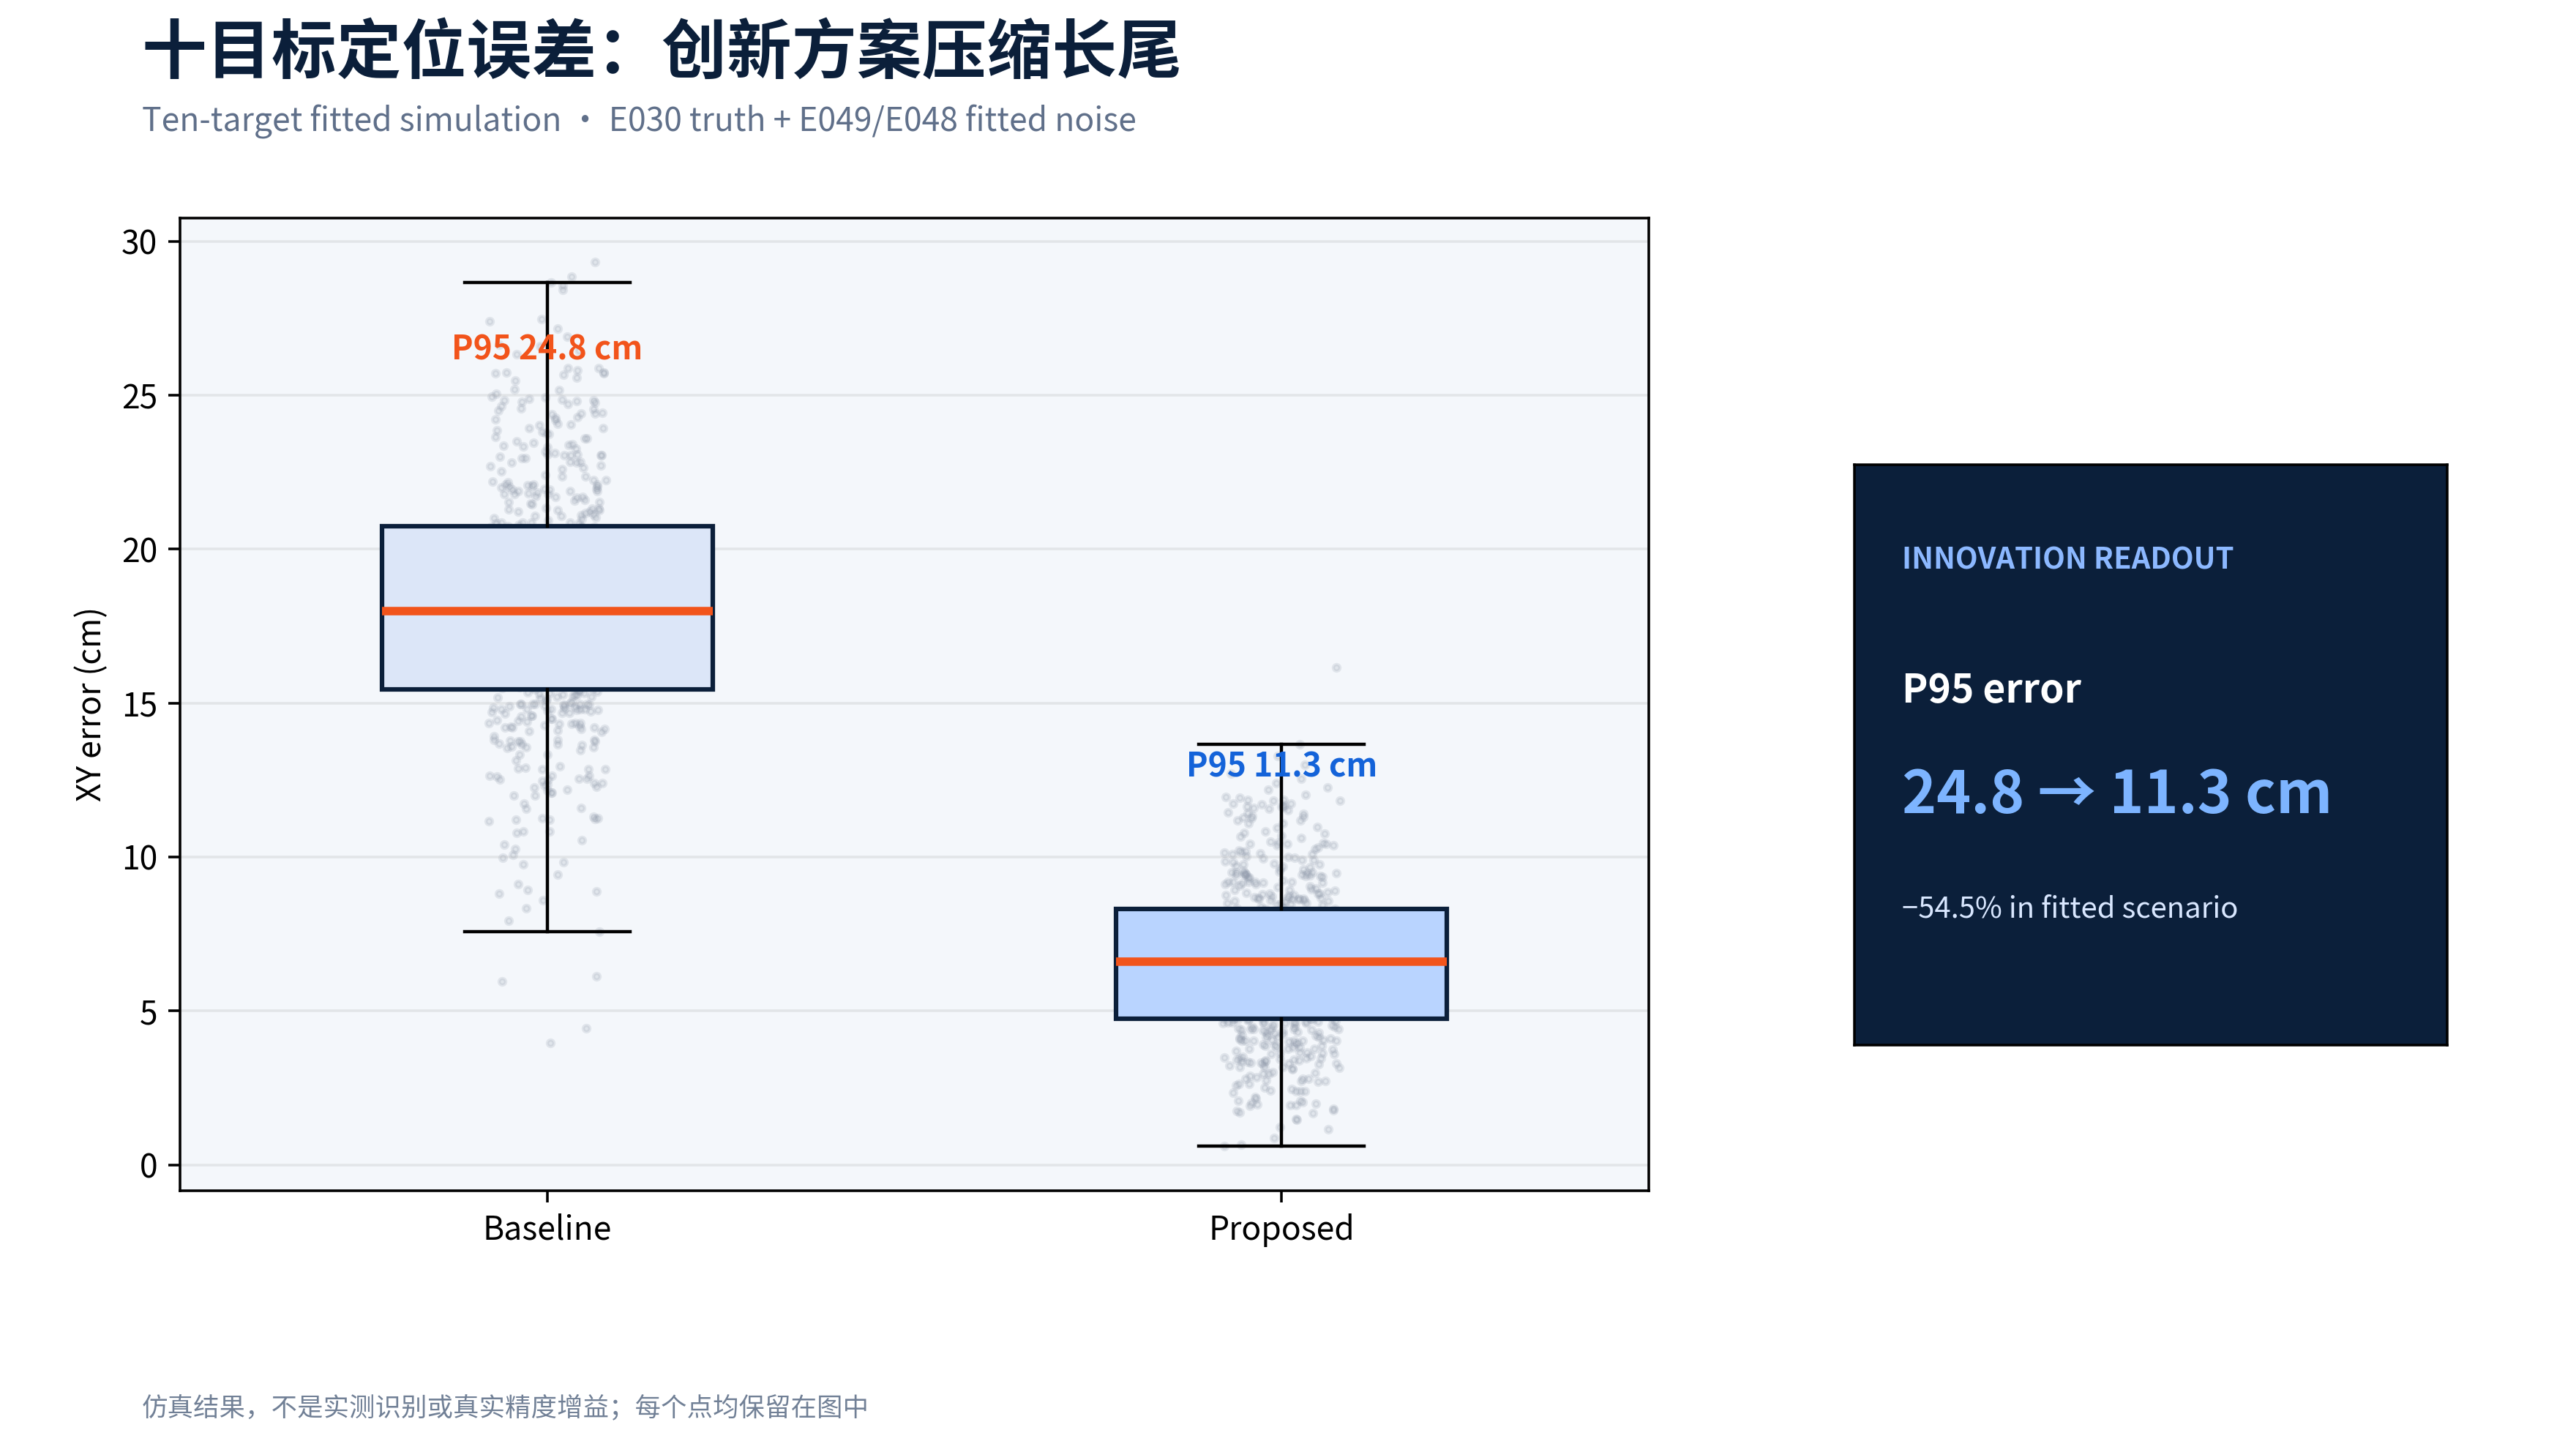
\includegraphics[width=0.94\textwidth]{assets/fig_ten_target_error_box_v01.png}
  \caption{E050 十目标拟合仿真的二维定位误差分布}\label{fig:fitted-error}
\end{figure}

\subsubsection{实时性、帧率与端到端延迟}
我们在 E042 的静置采集中获得 34021 条 \texttt{SCALED\_IMU} 消息，持续 180.0 s，平均频率为 189.0 Hz，源采样间隔位于 5--15 ms，未出现超过 50 ms 的缺口。源时钟相对接收时钟的拟合漂移约为 $-20.42$ ppm，接收时间残差的 $99\%$ 分位数约为 7.24 ms。这些结果表明，静置条件下 IMU 数据流能够以较稳定的频率进入采集链路，为同步和离线回放提供基础。

上述时间拟合只反映源时钟与接收时钟之间的相对关系，不能推导出传感器的绝对端到端延迟。将飞控姿态变化与 IMU 变化进行对比时，主要运动轴的相关系数约为 0.95--0.99，最佳相对时差位于 $-5$ 至 10 ms 范围内。由于飞控姿态仍是相关估计而非外部真值，我们只将该结果作为信号变化一致性的证据，不把它包装为独立的姿态精度或 UWB 时延验证结果。

\subsubsection{稳定性与连续运行表现}
我们同样保留了真实运动回放中的失败现象。回放中发现两处源 IMU 缺口，分别约为 500 ms 和 70 ms；系统会跳过缺口处的角积分并将该段标记为不完整，而不通过插值或放宽门限掩盖问题。偏航回放的估计器累计耗时约为 382.7 s，超过约 178 s 的数据时长，说明当前近似配置尚不满足该段的实时性要求。该结果表明，软件主链路的稳定性已可通过受控测试验证，而真实平台融合的连续性与实时性仍需进一步优化和复验。

\subsubsection{资源占用}
当前运行记录尚未形成可用于横向比较的 CPU、内存和设备端功耗统计，因此我们不在报告中虚构资源占用数字。现有的 382.7 s 回放耗时说明，当前平台估计器的处理效率仍是需要重点关注的工程问题。后续我们将补充统一硬件平台上的 CPU 利用率、峰值内存、模型推理耗时和端到端延迟测试，以在定位精度与部署成本之间形成可量化的权衡依据。

\subsection{测试结果与分析}
\subsubsection{已验证的软件/仿真结果}
E044 的 192 个 ROS2 测试用例和 11 个 Web 契约测试均通过，覆盖目标注册、身份关联、多帧几何接口、融合状态和可视化输出。E050 的误差统计和图\ref{fig:fitted-error}则展示了明确拟合假设下的误差分布变化。两类结果说明，我们的主链路已经具备可测试、可追溯的实现基础，且方案原型在受控噪声情景下呈现出更小的二维误差和更短的误差长尾。

\subsubsection{实机结果（仅在具备可追溯实验记录时写入）}
我们已完成真实 IMU 数据采集和基础质量检查，确认静置条件下数据频率、时间连续性和主要运动轴信号相关性具备分析条件。但实机平台融合的连续性与实时性尚未通过验收，且尚未取得包含真实目标注册、有效多帧几何、平台位姿和最终 \texttt{map} 坐标输出的同一次闭环录包。因此，本节不报告实机端到端定位误差，而将其保留为下一阶段的验收目标。

\subsubsection{结果对比与误差来源分析}
仿真中的误差差异来自视觉残差、平台位姿传播、UWB 测距和几何观测条件的共同作用。在 E050 的拟合设定中，方案原型以更小的残差与偏差尺度得到较低的中位误差、$P95$ 误差和 $RMSE$，说明长尾项会明显影响最终定位。真实系统中的锚点测量、相机内外参、初始位姿、相机视角、目标纹理和运动基线同样会改变误差分布；我们将在后续录包中逐项控制这些因素，并借助独立真值区分算法、标定和传感器误差。

\subsection{当前限制与改进方向}
当前的限制集中在真实联合验收尚未闭环：平台近似配置、IMU 话题接入、初始位姿来源和真实目标米制几何尚未在同一次实机运行中完整验证；运动数据中的 IMU 缺口、UWB 时延和估计器实时性问题也需继续定位。下一阶段，我们将完成锚点、相机与初始位姿核验，采集图像、\texttt{CameraInfo}、IMU、原始 UWB 距离和平台状态的同步数据并离线回放；随后以独立真值评估误差、时延、连续运行和异常恢复能力，再将软件级和仿真级结论升级为实机性能结论。

\section{团队分工、总结与展望}\label{sec:team}
\subsection{团队组织与协作机制}
我们采用“算法复现、硬件联调、系统展示和测试归档”并行推进的协作方式。组长负责总体技术路线和关键算法的衔接，各成员围绕明确的模块边界开展工作，并通过 ROS2 消息接口、配置文件、实验记录和图表源文件完成交接。每当一个阶段形成结果，我们都会同步记录输入数据、代码版本、运行编号和结论边界，以减少不同模块之间的信息断层，也使报告中的设计、操作步骤和测试结果可以相互对应。

\subsection{成员分工与具体贡献}

\begin{table}[htbp]
  \centering
  \small
  \caption{团队成员分工与具体贡献}\label{tab:team-division}
  \begin{tabular}{p{2.3cm}p{3.0cm}p{6.1cm}}
    \toprule
    成员 & 负责内容 & 交付物与协作接口 \\
    \midrule
    王博（组长） & GDR-Net 复现架构与核心算法优化 & 搭建 GDR-Net 复现架构，统筹核心算法优化与技术路线衔接 \\
    李喆 & 硬件联调与 UWB 代码 & 负责硬件联调、UWB 数据接入及相关代码实现与验证 \\
    胡艺琳 & LightGlue 复现、网页与测试 & 负责 LightGlue 复现，参与网页功能和测试工作 \\
    阳宇 & 硬件安全、PPT 与网页制作 & 负责硬件安全保障、PPT 制作，并参与网页制作 \\
    吴嘉莹 & SuperPoint 复现 & 负责 SuperPoint 特征提取模块的复现与接入 \\
    \bottomrule
  \end{tabular}
\end{table}

\subsection{项目实施过程与问题解决}
在项目实施过程中，我们先完成 GDR-Net、LightGlue 和 SuperPoint 等视觉模块的复现与接入，再围绕 UWB、IMU 和相机数据推进硬件联调，并同步建设网页展示、PPT 材料和实验测试流程。这样的推进方式使算法模块能够独立迭代，也使硬件输入、展示界面和测试记录逐步汇入同一定位主链路。

真实系统接入阶段，我们没有回避数据质量和启动条件带来的问题。面对 IMU 数据缺口、近似配置无法直接通过统一入口加载、平台初始位姿不足以及实机目标几何尚未闭环等情况，我们保留失败记录和限制说明，而非用合成数据或界面演示替代实机结论。通过将这些问题拆分为数据接入、标定、初始化、几何观测和性能验证等环节，我们明确了后续补验的顺序，也降低了多人协作中重复排查的成本。

\subsection{项目总结}
我们围绕无人机平台状态与外部静态目标定位两个对象，构建了从视觉、UWB 和惯性数据接入，到坐标转换、多帧几何、融合估计、可视化和记录归档的整体框架。平台定位与目标定位在统一 \texttt{map} 坐标系中协同，定位链路保持只读，不直接干预飞行控制，从而明确了实验系统的功能边界。

本次实训的收获不仅在于完成了多个开源视觉模块和定位接口的复现与集成，更在于形成了可分层验证的工作方法。当前软件级测试已经覆盖消息通信、静态目标约束、状态管理、网页展示和记录接口；运行编号、配置副本、数据散列和测试结果之间的关联，使我们能够回溯每一项结论的来源。已有结果支持“软件主链路和部分真实传感器采集能力已经得到验证”的判断，也支持“在指定拟合情景下，误差模型缩放会改变二维误差分布”的分析。

\subsection{不足与后续工作}
我们也清楚地认识到，当前证据尚不足以宣称已经获得实机端到端定位精度、实时性或飞行稳定性。后续工作将围绕真实联合验收展开：首先完成 UWB 锚点、相机外参和平台初始位姿的独立测量与配置核验；其次采集包含图像、\texttt{CameraInfo}、IMU、原始 UWB 距离和平台状态的同步数据，并完成真实目标从网页注册到 \texttt{map} 坐标输出的连续录包；最后结合独立真值，对二维与三维误差、端到端延迟、连续运行能力和异常恢复能力进行统一评估。完成这些工作后，我们才能将软件级和仿真级结论稳妥地升级为系统性能验收的实机结论。

\begin{thebibliography}{99}
  \bibitem{ros2} Open Robotics. ROS 2 Documentation[EB/OL]. \url{https://docs.ros.org/}.
  % 请按实际引用的论文、开源项目与技术文档补充参考文献，勿列入未实际使用的资料。
\end{thebibliography}

\clearpage
\appendix
\section*{附录}
\addcontentsline{toc}{section}{附录}
\section{关键配置与接口表}
\subsection{沙盘真值坐标与坐标系约定}
本报告中用于十目标误差分析的真值来自 E030 的用户接受实体沙盘登记表，坐标系为 \texttt{physical\_sandbox\_map\_v01}：以沙盘指定桌角为原点，采用右手系，$x$ 轴沿桌面宽度、$y$ 轴沿桌面长度、$z$ 轴向上，单位均为 m。表\ref{tab:sandbox-ten-truth}列出 E050 实际纳入评估的全部 10 个交通灯目标；它们构成本文“十目标”仿真的完整真值点集，而不是对整座沙盘全部物体的重新测量。

\begin{longtable}{p{3.2cm}ccc}
\caption{E050 十目标仿真的完整沙盘真值点（\texttt{map}，m）}\label{tab:sandbox-ten-truth}\\
\toprule
目标 ID & $x_{\mathrm{truth}}$ & $y_{\mathrm{truth}}$ & $z_{\mathrm{truth}}$ \\
\midrule
\endfirsthead
\toprule
目标 ID & $x_{\mathrm{truth}}$ & $y_{\mathrm{truth}}$ & $z_{\mathrm{truth}}$ \\
\midrule
\endhead
J01-NW-HIGH & 0.0788 & 0.9670 & 0.2200 \\
J01-NE-HIGH & 0.9062 & 0.9670 & 0.2200 \\
J01-SE-HIGH & 0.9062 & 0.0841 & 0.2200 \\
J01-SW-HIGH & 0.0788 & 0.0841 & 0.2200 \\
J02-NW-HIGH & 0.0788 & 2.9114 & 0.2200 \\
J02-NE-HIGH & 0.9062 & 2.9114 & 0.2200 \\
J02-SE-HIGH & 0.9062 & 2.0286 & 0.2200 \\
J02-SW-HIGH & 0.0788 & 2.0286 & 0.2200 \\
J03-NW-HIGH & 3.0338 & 0.9670 & 0.2200 \\
J03-NE-HIGH & 3.8612 & 0.9670 & 0.2200 \\
\bottomrule
\end{longtable}

\subsection{坐标转换关系}
当 UWB 为平台提供距离约束、视觉负责观测机外静态目标时，目标位置通过平台位姿和相机外参进入世界坐标系。其基本关系为
\[
{}^{\mathrm{map}}\mathbf{p}_{\mathrm{target}}
= {}^{\mathrm{map}}\mathbf{T}_{\mathrm{base\_link}}
  {}^{\mathrm{base\_link}}\mathbf{T}_{\mathrm{camera}}
  {}^{\mathrm{camera}}\mathbf{p}_{\mathrm{target}} .
\]
其中，${}^{\mathrm{camera}}\mathbf{p}_{\mathrm{target}}$ 来自视觉检测、匹配与多帧几何；${}^{\mathrm{map}}\mathbf{T}_{\mathrm{base\_link}}$ 是动态平台位姿；${}^{\mathrm{base\_link}}\mathbf{T}_{\mathrm{camera}}$ 是由安装与标定确定的静态外参。UWB 默认约束平台而非外部目标，因此不能把 UWB 原始距离直接写作目标的 \texttt{map} 坐标。若未来采用 UWB 直接测量目标，还必须单独登记 UWB 标签到 \texttt{target\_link} 的外参。

\begin{longtable}{p{3.7cm}p{3.3cm}p{4.8cm}}
\caption{目标坐标转换链及其标定要求}\label{tab:coordinate-chain}\\
\toprule
变换/量 & 语义与来源 & 使用约束 \\
\midrule
\endfirsthead
\toprule
变换/量 & 语义与来源 & 使用约束 \\
\midrule
\endhead
\texttt{map} $\rightarrow$ \texttt{base\_link} & 平台在沙盘参考系下的动态位姿；由平台定位链路发布 & 应记录时间戳和来源；缺失时不应发布伪造的目标世界坐标。\\
\texttt{base\_link} $\rightarrow$ \texttt{camera} & 无人机机体至相机光学坐标系的静态外参 & 必须由安装/标定记录给出；不得仅依据 frame 名称推断轴向。\\
\texttt{camera} $\rightarrow$ \texttt{target\_link} & 视觉观测得到的目标相对位置或射线几何 & 使用相机内参和有效观测；静态目标需通过身份一致性约束跨帧关联。\\
\texttt{map} $\rightarrow$ \texttt{target\_link} & 面向展示与评估的最终目标状态 & 统一使用 m 和右手系；输出附带质量、来源和历史状态。\\
\bottomrule
\end{longtable}

\begin{longtable}{p{3.0cm}p{3.6cm}p{5.2cm}}
\caption{关键配置与接口说明}\label{tab:appendix-interface}\\
\toprule
类别 & 代表性内容 & 使用说明 \\
\midrule
\endfirsthead
\toprule
类别 & 代表性内容 & 使用说明 \\
\midrule
\endhead
输入接口 & 图像、\texttt{CameraInfo}、IMU、UWB 原始距离、平台状态 & 记录消息来源、时间戳、坐标系和物理单位。\\
标定配置 & 相机内外参、UWB 锚点坐标、平台与相机安装关系 & LIVE 模式应使用实际标定文件；变更后需重新核验。\\
核心输出 & \texttt{map} 坐标系下的平台/目标状态、质量标记、历史状态 & 输出需说明是当前观测、历史保留还是重新识别结果。\\
归档信息 & 运行编号、配置副本、代码版本、输入数据位置与校验信息 & 用于结果回放、问题定位和结论追溯。\\
\bottomrule
\end{longtable}

\section{主要操作命令}
以下命令为统一定位入口的使用示例。实际运行前应以本次实验的工作空间、配置路径和设备状态为准，并先完成第\ref{sec:usage}章所述核验。
\begin{verbatim}
ros2 launch dual_localization dual_localization.launch.py
ros2 topic list
ros2 bag record <required_topics>
ros2 bag play <recorded_bag>
\end{verbatim}

\section{测试用例/结果汇总}
\subsection{十目标真值、模拟估计坐标与误差统计}
E050 以表\ref{tab:sandbox-ten-truth}的真值为固定输入，对每个目标、每种方法各生成 60 帧观测。表\ref{tab:ten-target-estimate}给出其中 ``proposed'' 拟合仿真方案的逐目标估计均值、平均二维误差和 $P95$ 二维误差；估计仅有 $x$、$y$ 分量，$z$ 值并未由该仿真产生。表中的数值由可追溯文件 \texttt{tbl\_ten\_target\_simulated\_observations\_v01.csv} 的完整 1200 行记录汇总得到，不是实机识别或实测定位坐标。

\begin{longtable}{p{2.7cm}p{2.7cm}p{2.8cm}cc}
\caption{E050 十目标的模拟估计坐标与二维误差统计（proposed，m）}\label{tab:ten-target-estimate}\\
\toprule
目标 ID & 真值 $(x,y,z)$ & 模拟估计均值 $(\bar{x},\bar{y})$ & 平均 $e_{xy}$ & $P95$ $e_{xy}$ \\
\midrule
\endfirsthead
\toprule
目标 ID & 真值 $(x,y,z)$ & 模拟估计均值 $(\bar{x},\bar{y})$ & 平均 $e_{xy}$ & $P95$ $e_{xy}$ \\
\midrule
\endhead
J01-NW-HIGH & (0.0788, 0.9670, 0.2200) & (0.0342, 0.9306) & 0.0653 & 0.1142 \\
J01-NE-HIGH & (0.9062, 0.9670, 0.2200) & (0.8638, 0.9189) & 0.0679 & 0.1024 \\
J01-SE-HIGH & (0.9062, 0.0841, 0.2200) & (0.8643, 0.0411) & 0.0670 & 0.1111 \\
J01-SW-HIGH & (0.0788, 0.0841, 0.2200) & (0.0440, 0.0374) & 0.0640 & 0.1163 \\
J02-NW-HIGH & (0.0788, 2.9114, 0.2200) & (0.0438, 2.8661) & 0.0638 & 0.1165 \\
J02-NE-HIGH & (0.9062, 2.9114, 0.2200) & (0.8659, 2.8683) & 0.0660 & 0.1061 \\
J02-SE-HIGH & (0.9062, 2.0286, 0.2200) & (0.8684, 1.9841) & 0.0644 & 0.1051 \\
J02-SW-HIGH & (0.0788, 2.0286, 0.2200) & (0.0397, 1.9874) & 0.0652 & 0.1040 \\
J03-NW-HIGH & (3.0338, 0.9670, 0.2200) & (2.9895, 0.9194) & 0.0718 & 0.1136 \\
J03-NE-HIGH & (3.8612, 0.9670, 0.2200) & (3.8215, 0.9185) & 0.0682 & 0.1145 \\
\bottomrule
\end{longtable}

图\ref{fig:appendix-ten-target-overlay}用星标表示 10 个固定真值点，并叠加 ``proposed'' 情景下的模拟估计轨迹。星标与点云之间的系统性偏移对应表\ref{tab:ten-target-estimate}中的均值偏差；点云的离散程度反映帧级拟合噪声，而不是无人机在真实沙盘中的飞行轨迹或在线输出。
\begin{figure}[H]
  \centering
  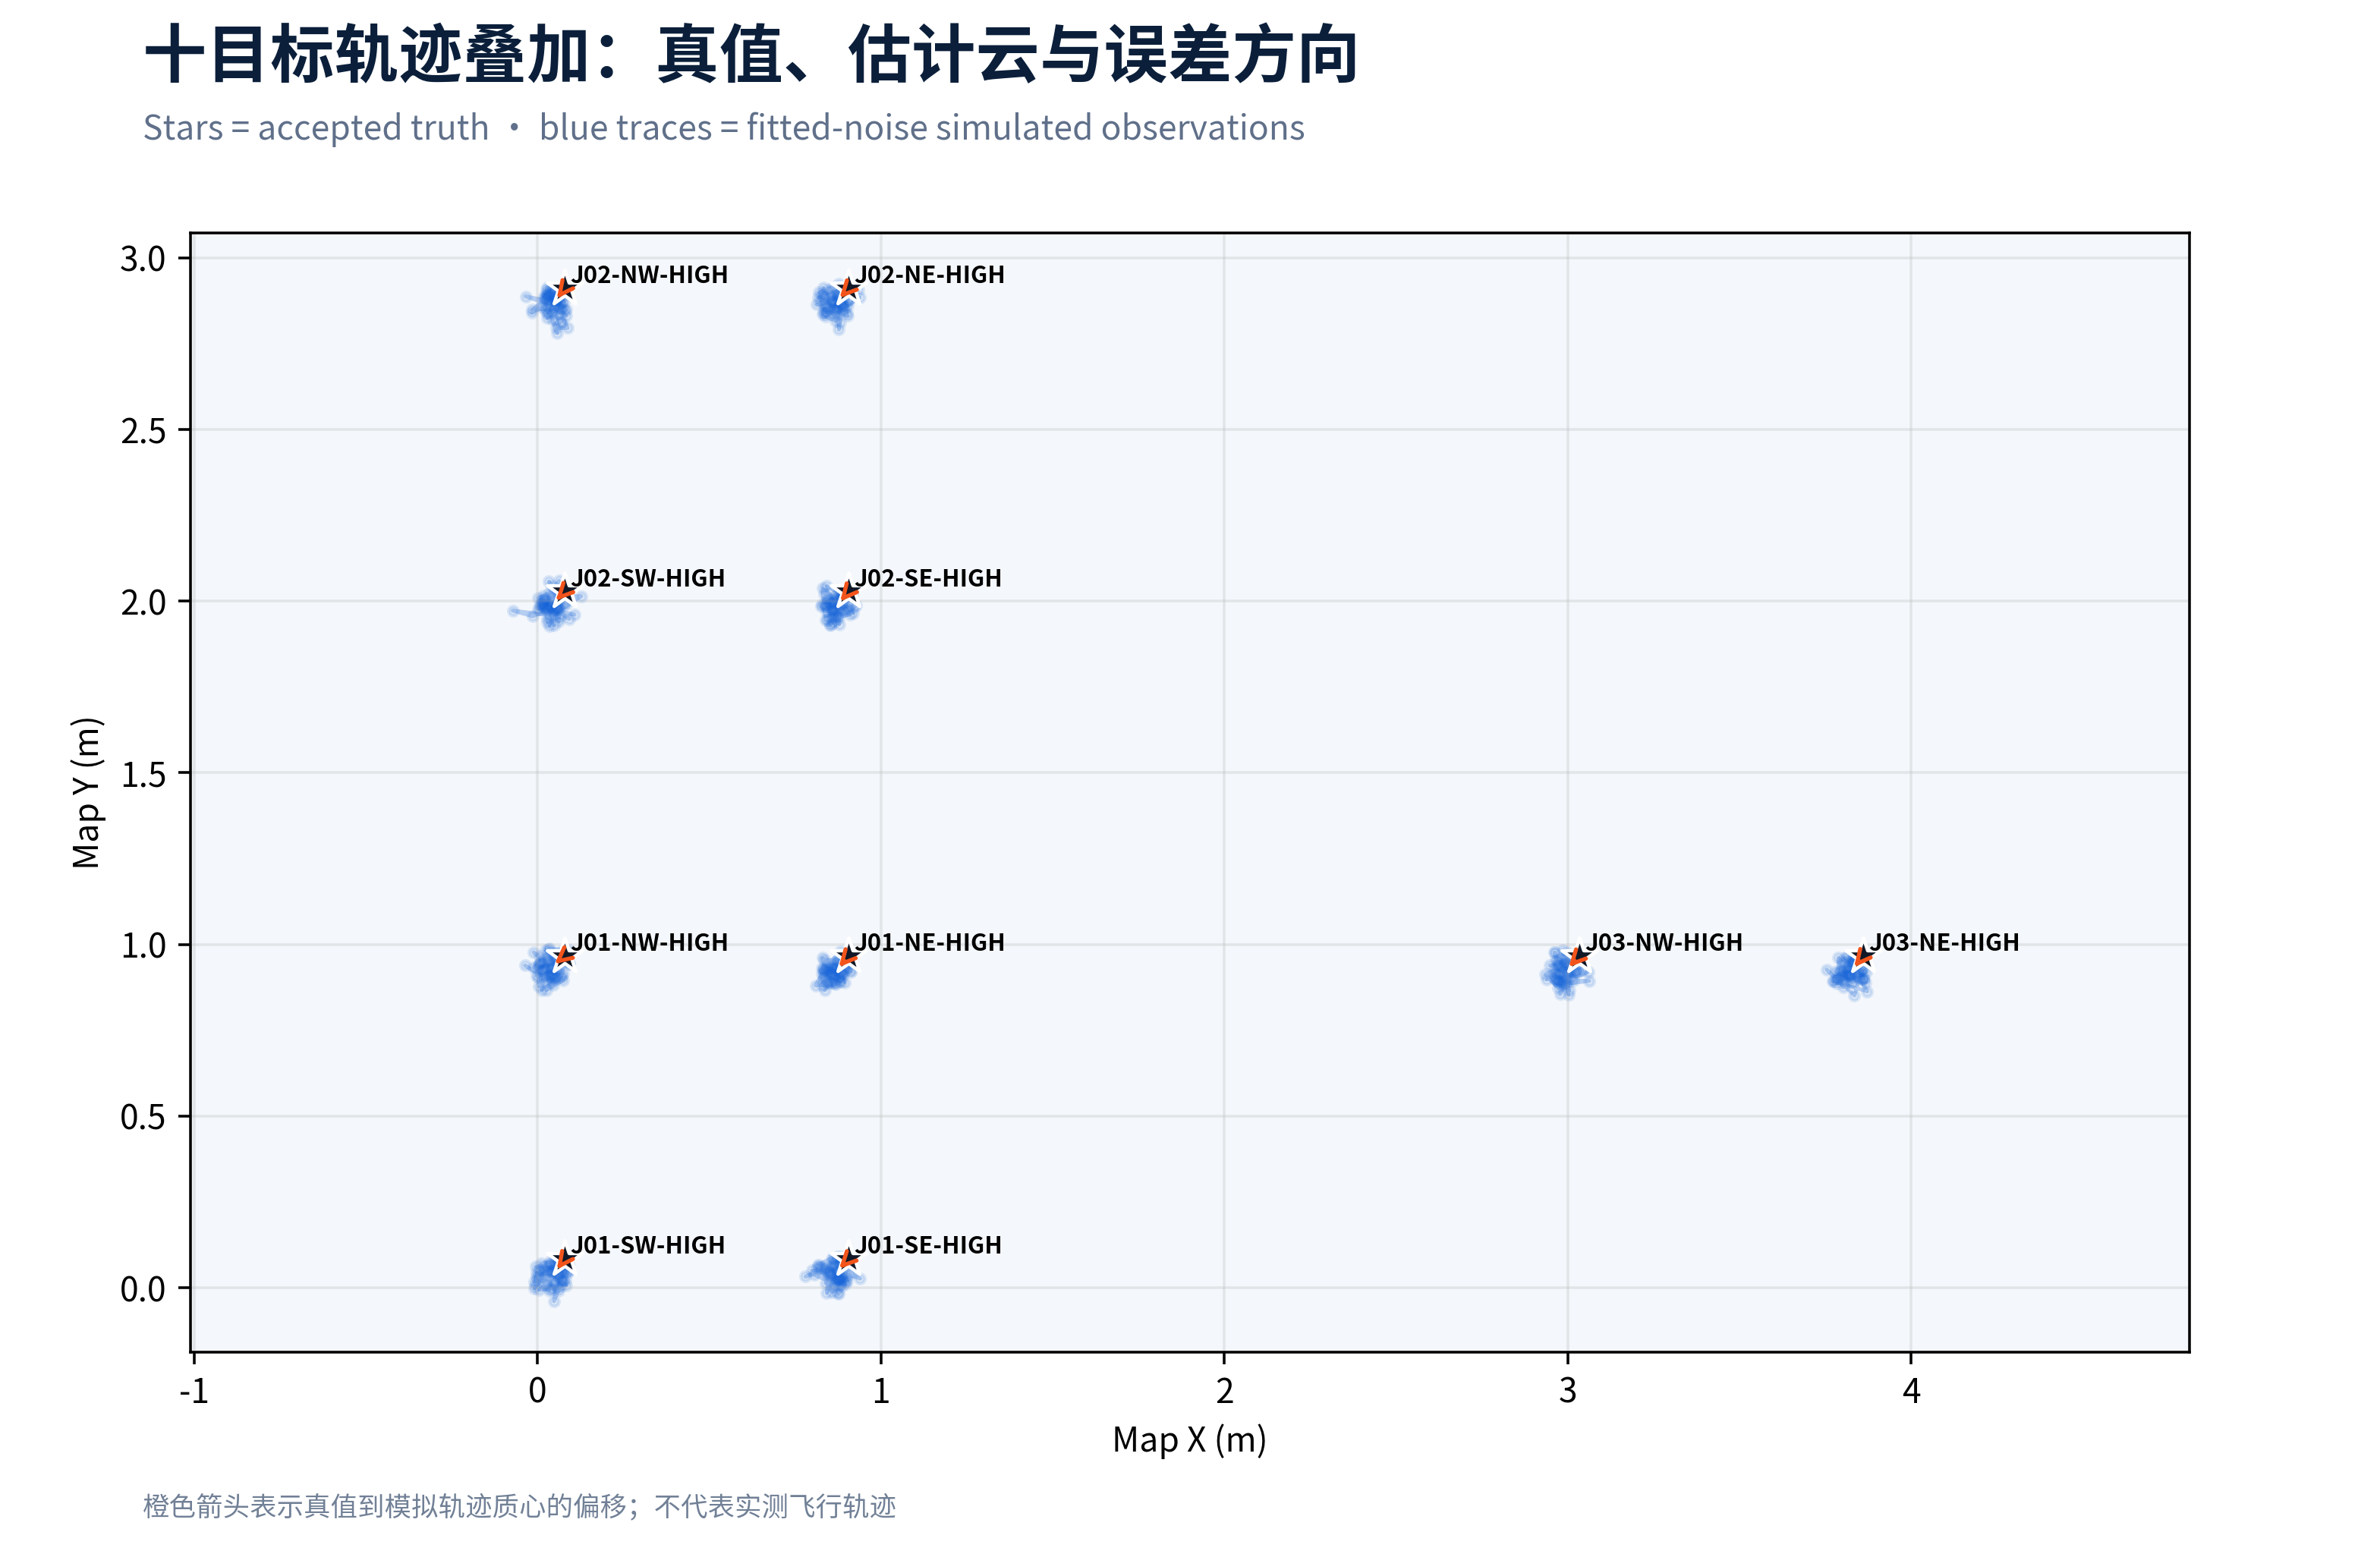
\includegraphics[width=0.94\textwidth]{assets/fig_ten_target_trajectory_overlay_v01.png}
  \caption{E050 十目标真值点与 proposed 拟合仿真估计轨迹叠加图}\label{fig:appendix-ten-target-overlay}
\end{figure}

图\ref{fig:appendix-error-distribution}展示同一 E050 数据集的完整 1200 条帧级二维误差分布：每种方法各 600 条记录。箱体、须线与散点共同呈现误差中心、离散范围和长尾；它用于说明声明的残差与偏差缩放如何改变拟合仿真分布，不能作为实机算法提升或真实端到端精度的证明。
\begin{figure}[H]
  \centering
  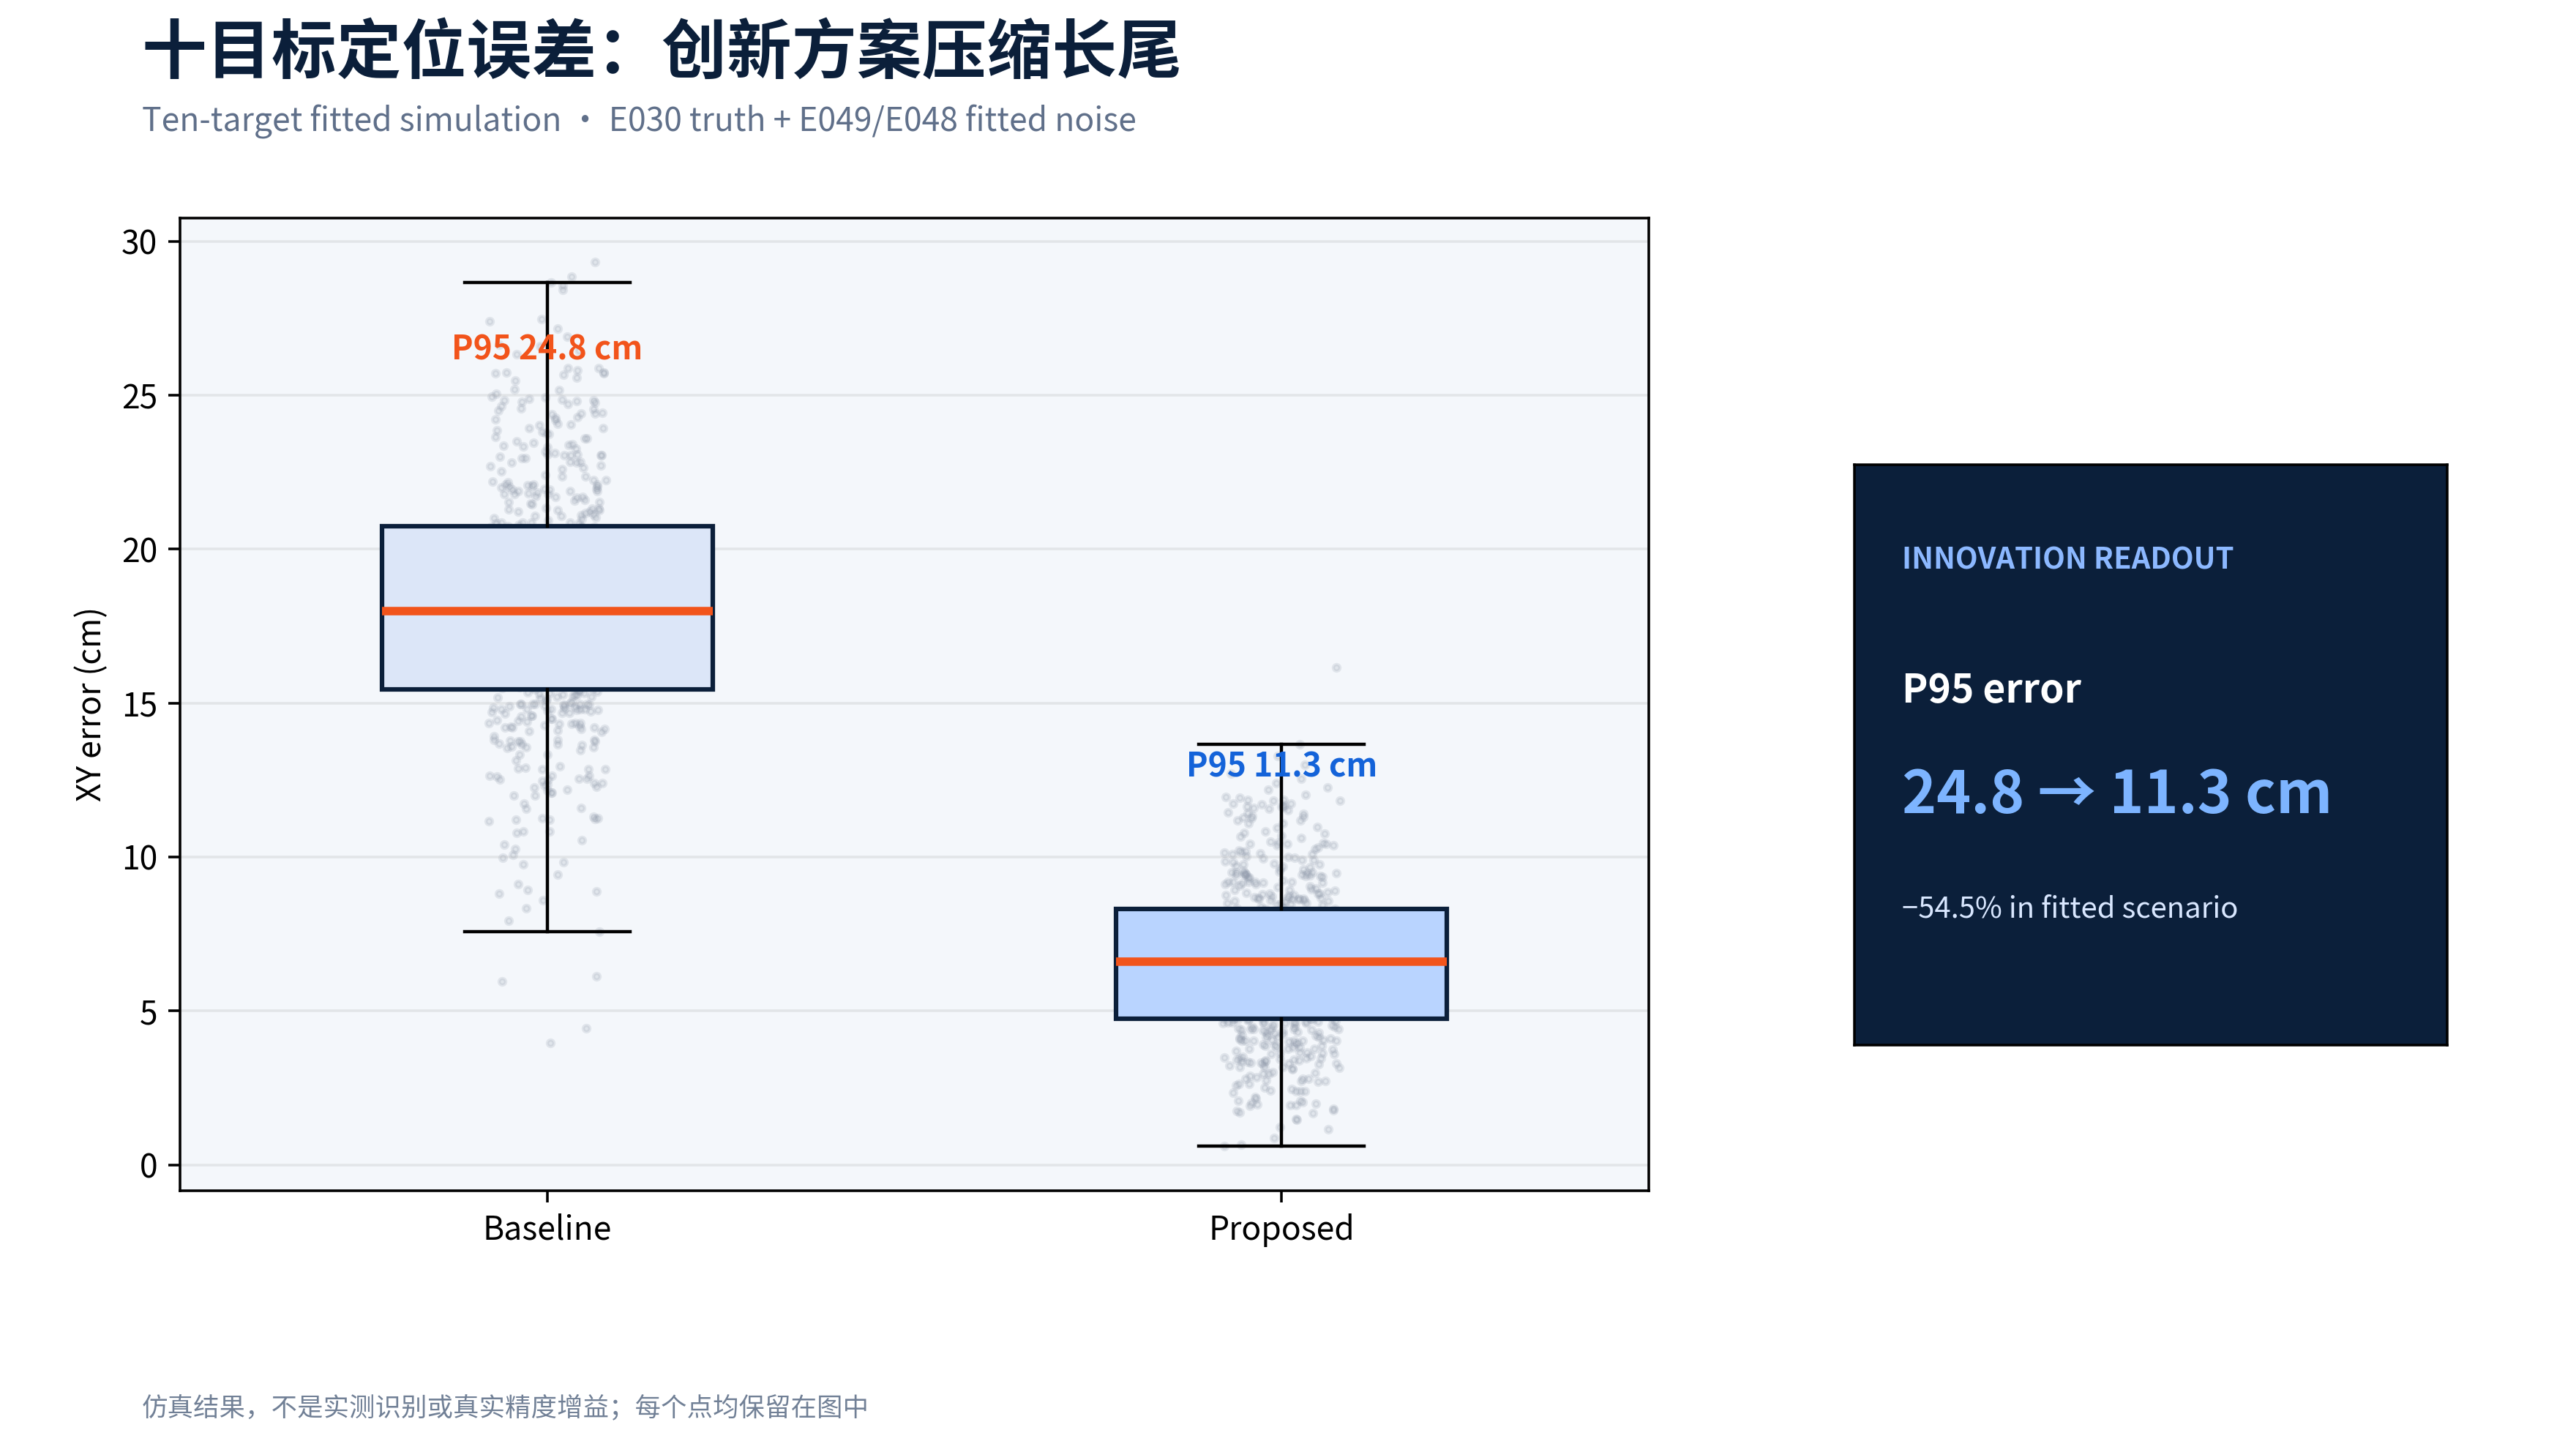
\includegraphics[width=0.94\textwidth]{assets/fig_ten_target_error_box_v01.png}
  \caption{E050 全部 1200 条拟合仿真观测的二维误差分布}\label{fig:appendix-error-distribution}
\end{figure}

\begin{table}[htbp]
  \centering
  \caption{当前测试证据汇总}
  \begin{tabular}{p{3.1cm}p{3.5cm}p{5.2cm}}
    \toprule
    验证类别 & 已有证据 & 可支撑的结论边界 \\
    \midrule
    软件功能测试 & E044：192 个 ROS2 测试、11 个 Web 契约测试通过 & 软件接口、状态管理和展示契约具备可测试基础。\\
    真实传感器采集 & E042：静置 IMU 数据频率与时间连续性检查 & 支撑数据采集链路的基础质量分析，不等同于端到端定位验收。\\
    拟合仿真分析 & E050：十目标二维误差分布统计 & 支撑指定假设下的误差分布分析，不等同于实机精度。\\
    实机联合验收 & 尚未形成可追溯的完整闭环记录 & 不报告端到端实机精度、实时性或稳定性结论。\\
    \bottomrule
  \end{tabular}
\end{table}

\section{成员贡献说明}
本项目由王博（组长）、李喆、胡艺琳、阳宇和吴嘉莹共同完成。王博负责 GDR-Net 复现架构的搭建与核心算法优化；李喆负责硬件联调和 UWB 相关代码；胡艺琳负责 LightGlue 的复现、网页和测试；阳宇负责硬件安全、PPT 制作和网页制作；吴嘉莹负责 SuperPoint 的复现。具体分工及协作方式见第\ref{sec:team}章。

\end{document}
